

\section{Project Proposal}
The aim of this project is to design and develop a mathematical model of the most important macroeconomic indicators in the Russian national economy.
The model will be mainly inspired from the macroeconomic model designed and used by the Office of Budget Responsibility (OBR) in the UK \parencite{obr}.
Such model is important for various reasons.
The OBR uses its model for forecasting%
\footnote{\url{https://obr.uk/forecasts-in-depth}}.
They prepare and publish economic forecasts for the purposes of forecasting the public finances \parencite{obr2}.
Examine figure \ref{img:oil-prices} for an example about their forecasting.

\begin{figure}[!htb]
\centering
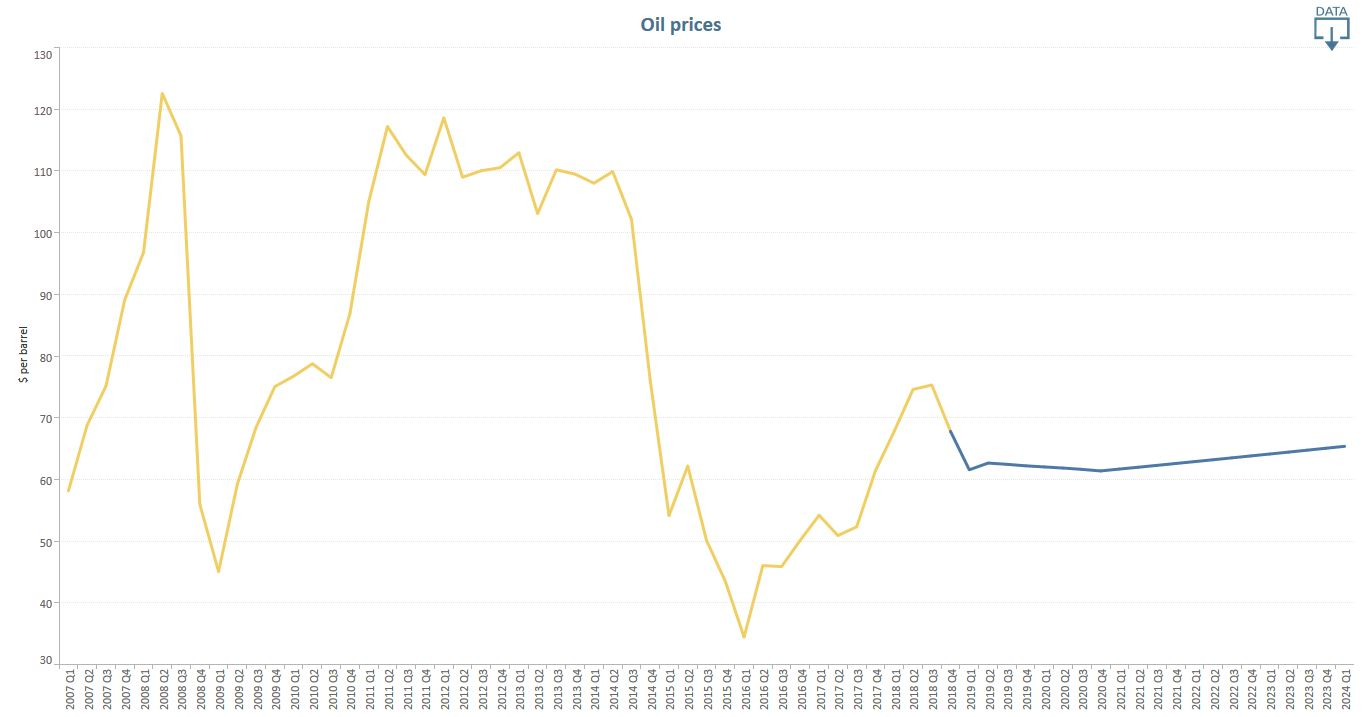
\includegraphics[width=1\textwidth]{images/oil-prices.jpg}
\caption{%
UK oil price forecasting by OBR\protect\footnotemark.
The yellow part corresponds to the outturn (real) price recorded,
while the blue part corresponds to the forecasting (predicted) price.
$Q_i$ on the horizontal axis corresponds the $i^{th}$ quarter of the year.
}
\label{img:oil-prices}
\end{figure}

\footnotetext{\url{https://obr.uk/forecasts-in-depth/the-economy-forecast/conditioning-assumptions/\#oilprices}}




\subsection{Project Plan}
Table \ref{tbl:plan} describes the plan that will be used to accomplish this project.

\newcommand{\myColumnWidth}{\linewidth}
\newcolumntype{L}{>{\centering\arraybackslash}p{0.75\linewidth}}

\begin{table}[!htb]
\centering
\setlength{\tabcolsep}{0.5em} % for the horizontal padding
\renewcommand{\arraystretch}{2.4}% for the vertical padding
\begin{tabular}{|c|c|L|}
\hline
\textbf{Iteration}            & \textbf{Week} & \textbf{Tasks}                                   \\ \hline
\multirow{2}{*}{N/A} & 1    & \multirow{2}{*}{N/A}                                                 \\ \cline{2-2}
                     & 2    &                                                                      \\ \hline
\multirow{2}{*}{1} & 3  & \parbox{\myColumnWidth}{Write project proposal and plan. Review OBR model. Review common macroeconomic indicators.}                                \\ \cline{2-3} 
& 4  & \multirow{3}{*}{\parbox{\myColumnWidth}{Design a system of ordinary differential equations (ODEs) to provide dynamics for the model. Review macroeconomic indicators in more depth.}} \\ \cline{1-2}
\multirow{2}{*}{2}   & 5    &                                                                      \\ \cline{2-2}
                     & 6    &                                                                      \\ \hline
\multirow{2}{*}{3}   & 7    & Review and collect Russian economic statistics.                      \\ \cline{2-3} 
                     & 8    & Mid-term presentation.                                               \\ \hline
\multirow{2}{*}{4} & 9  & \multirow{2}{*}{Implement the model and numerically solve the ODEs system.}                                                \\ \cline{2-2}
                     & 10   &                                                                      \\ \hline
\multirow{2}{*}{5}   & 11   & Evaluate the model.                                                  \\ \cline{2-3} 
                     & 12   & \parbox{\myColumnWidth}{Improve the model, or enhance the model (e.g. introduce stochastic terms).} \\ \hline
\multirow{2}{*}{6} & 13 & \multirow{2}{*}{Iterate between improving and evaluating the model.}                                                           \\ \cline{2-2}
                     & 14   &                                                                      \\ \hline
N/A                  & 15   & Final presentation.                                                  \\ \hline
\end{tabular}
\caption{Project plan.}
\label{tbl:plan}
\end{table}



\subsection{Iterations}
This sections describes the actual work done in each iteration.

\subsubsection{Iteration 1}
\begin{itemize}
\item Did relevant reading of chapters 6 and 7 from \parencite{economics-book}.
\item Reviewed OBR.
\item Wrote project proposal.
\item Wrote project plan.
\end{itemize}

\subsubsection{Iteration 2}
\begin{itemize}
\item Did relevant reading of chapters 19 and 20 from \parencite{economics-book}.
\item Wrote proposed model section.
\item Familiarizing myself by reviewing some Russian economic statistics.
\end{itemize}
